\documentclass[a4paper,12pt]{article}

\usepackage{titlesec} %za renewcommand
\usepackage{titling} %za renewcommand
\usepackage{ragged2e} %za na pr. flushleft
\usepackage{fancyhdr}
\usepackage{enumitem}
\usepackage{pdflscape}
\usepackage{array}
%\usepackage{tabularx}
\usepackage{makecell} %multiline cells + other non multiline cell are centered horiz. and vert.
\usepackage[table]{xcolor}
\usepackage{geometry}
\usepackage{hyperref}
\usepackage{booktabs}
\usepackage{color, soul}
\usepackage{gensymb}
\usepackage{graphicx}
\usepackage{verbatim} %comment sections
\usepackage{makecell}


\usepackage{array}                                                                                                                                               
\newcolumntype{L}[1]{>{\raggedright\let\newline\\\arraybackslash\hspace{0pt}}m{#1}}
\newcolumntype{C}[1]{>{\centering\let\newline\\\arraybackslash\hspace{0pt}}m{#1}}
\newcolumntype{R}[1]{>{\raggedleft\let\newline\\\arraybackslash\hspace{0pt}}m{#1}}

\geometry{left=1.5cm,right=1.5cm,top=2cm,bottom=2cm}

\setcounter{page}{0}
\setcounter{section}{-1}
\setcounter{secnumdepth}{4}

\titleformat{\paragraph}
{\normalfont\normalsize\bfseries}{\theparagraph}{1em}{}
\titlespacing*{\paragraph}
{0pt}{3.25ex plus 1ex minus .2ex}{1.5ex plus .2ex}

\pagestyle{fancy}
\fancyhf{}
\lfoot{Powerd by \LaTeX}
\cfoot{Verzija 1.4}
\rfoot{Stran: \thepage}

\newcommand{\mlc}[1]{\raisebox{0ex}{\makecell{#1}}}

\renewcommand{\headrulewidth}{0.5pt}
\renewcommand{\footrulewidth}{0.5pt}

\renewcommand{\maketitle}{
	\begin{center}
	{\huge\bfseries
	\thetitle}
	\end{center}

	\vspace{1cm}

	\centerline{\textbf{Naročnik: Šaj d.o.o.}}
	\centerline{\textbf{Vodja projekta: Anton Zhezhov}}

	\vspace{1cm}

	\leftline{\textbf{Začetek: 09.10.2019 } \hfill \textbf{Konec: 31.01.2020}}

	\vspace{4cm}

	\begin{center}
	
			\begin{tabular}{c|c|c|c}
					Ime in Priimek&Vloga	  &e - Naslov						&Opomba\\
				\hline
					Anton Zhezhov &Preverjanje&anton.zhezhov@student.um.si & 		\\
				\hline
					Žiga Zorc	  &Razvoj	  &ziga.zorc@student.um.si 	   &		\\
			\end{tabular}
	
	\end{center}
}

\let\oldtitleline\titleline
\renewcommand{\titleline}{\oldtitleline*}

\title{Projekt CSUPP}
\author{Anton Zhezhov}


\begin{document}

%underline color options for "paramteri"
\setul{0.6ex}{0.17ex}
\definecolor{Red}{rgb}{1,0.0,0.6}
\setulcolor{Red}



\maketitle

\setlength{\titlewidth}{16cm}

\newpage

\section{Naročnikove zahteve}
	\subsection{Splošne informacije}
			\begin{center}
				\begin{tabular}{c|c}
						Dokument & Verzija 1.0 \\
						\hline
						Naročnik & Šaj d.o.o. \\
						\hline
						Lokacija dokumenta & \href{https://github.com/antonzezov/OPI\_LV\_csupp/tree/master/doc01}{Github url} \\ %za zdaj ni public
						\hline
						Odgovorna oseba & Direktor podetja Šaj d.o.o. \\
				\end{tabular}
			\end{center}
	\subsection{Zahteve}
 
	\hspace{1em} V podjetju Šaj d.o.o. se ukvarjamo z razvojem inovativnih rešitev na področju 
	avtomatizacije in digitalizacije upravljanja poslovnih prostorov. Pri načrtovanju 
	naših rešitev dajemo velik poudarek na okoljsko trajnost, energetsko učinkovitost 
	ter ergonomičnost produktov, saj se zavedamo, da omenjene lastnosti pozitivno vplivajo 
	tako na izboljšano uporabniško izkušnjo kot na optimizacijo poslovanja skozi nižanje 
	stroškov.
	
	V podjetju smo prepoznali pomanjkanje rešitev, ki bi celovito naslovile 
	problem zastarelosti poslovnih prostorov. V ta namen načrtujemo razvoj centralnega 
	sistema za upravljanje poslovnega prostora, s čimer se nadejamo preboja na trg 
	in s tem izboljšanja poslovnega uspeha. Projekt že ima izoblikovano idejno zasnovo, 
	in sicer tako glede strojne opreme kot izgleda in funkcionalnosti. Sedaj smo v fazi 
	iskanja resnega partnerja, ki bi prevzel razvoj programske opreme. Ker želimo preveriti 
	osnovni koncept in delovanje centralnega sistema za upravljanje prostora, naj bo program 
	napisan v obliki simulatorja. Najprej potrebujemo preprost simulator brez grafičnega 
	vmesnika, ki bo izdelan kot konzolna aplikacija v jeziku C++ v integriranem razvojnem 
	okolju Visual Studio. Od simulatorja pričakujemo brezhibno in robustno delovanje v 
	operacijskem sistemu Windows. Poleg tega mora biti simulator hiter in preprost za uporabo. 
	Simulator naj omogoča krmiljenje temperature, vlage in osvetljenosti prostora. Predpogoj 
	je, da uporabnik v tekstovno datoteko vpiše želene ambientalne lastnosti v obliki: 
	
	TEMPERATURA: vrednost 

	VLAZNOST: vrednost v obliki relativne vlažnosti [\%] 

	OSVETLJENOST: vrednost v luksih [lx] 
	\\
	V datoteki naj bo še: 

	INTERVAL TEMPERATURE: [10,40]
	
	STOPNJA VLAZNOSTI: [30,60]

	INTERVAL OSVETLJENOSTI: [10,10000] 
	\\
	Simulator naj pred pričetkom prebere 
	vrednosti iz datoteke, nato pa naj omogoča izbiro med tremi načini delovanja: 

	1. Testni način: Uporabnik v program vnese dejansko temperaturo v prostoru. Računalnik vneseno 
	temperaturo pretvori v ostale relevantne merske enote. Nato naj izračuna razliko do 
	želene temperature (v vseh izbranih merskih enotah) in izvede ukaz za regulacijo 
	temperature. Analogno naj simulator omogoča vpis, izračun in izvedbo ukazov še za 
	vlažnost in osvetljenost. Simulacija se izvaja, dokler je ne prekine uporabnik. 
	
	2. Avtomatski način: Računalnik naj si izmisli dejansko temperaturo na intervalu 
	podanem v datoteki, pri čemer jo pretvori v najpomembnejše preostale merske enote. 
	Izmisli naj si še relativno stopnjo vlažnosti, in sicer med 30 in 60 \%, ter osvetljenost 
	na intervalu z datoteke. Nato naj za vsako posamezno meritev izračuna odstopanje od 
	želenih vrednosti ter izvede ukaze za popravek. Simulator naj izvede 100 meritev, pri 
	čemer izvede posamezno meritev vsake 3 sekunde. Na koncu simulacije naj izračuna 
	povprečno vrednost meritev ter povprečno odstopanje od želenih vrednosti za posamezne 
	\hyperlink{subsection.1.8}{\ul{parametre}}. 

	3. Avtomatski način 2: Simulator naredi isto kot v točki 2, pri čemer 
	naj uporabniku omogoča izbiro pri številu meritev in časovnem razmiku med njimi. 
	Izvajalec mora natančno slediti vsem internim standardom in poskrbeti za dokumentacijo. 
	
	Sestavni del projekta sta tudi razvijalska dokumentacija in uporabniški priročnik. 
	Od izvajalca pričakujemo, da do 24. 10. 2019 do 23.55 odda plan projekta, ki vključuje ceno. 
	Program in dokumentacija morata biti oddana najkasneje 23. 1. 2020 do 23.55. 
	Projekt bo plačan po posameznih zaključenih fazah. Za vsak teden zamude bo odbitih 10 \% plačila. 
	\\
	
	\leftline{Maribor 01.10.2019} 

	\hfill Direktor podjetja Šaj d.o.o.	

\newpage

\section{Plan projekta}

	\subsection{Tabela}

	\subsection{Kratek opis problema}

		\hspace{1em} Podjetje Šaj d.o.o. (v nadaljevanju naročnik) je dne 1. 10. 2019 naročilo 
		razvoj centralnega sistema za upravljanje poslovnega prostora.
		
		Naročnik želi optimizirati svoje poslovne prostore z avtomatiziranim sistemom, 
		ki meri in upravlja s paramteri. Sistem je preprost "simulator", ki je sposoben 
		prilagajanja \hyperlink{subsection.1.8}{\ul{parametrov}} tako avtomatsko kot na specifične uporabnikove zahteve.
		\subsubsection{Globalni cilji(globalne zahteve), ki jih želimo s produktom doseči}

		\begin{itemize}
				\item Izdelati simulator, ki primerno regulira {\hyperlink{subsection.1.8}{\ul{parametre}}} v prostoru
			\item Simulator mora biti hiter in preprost za uporabo
		\end{itemize}

		\subsubsection{Omejitve}

				\begin{itemize}
					\item Programski jezik: C++
					\item Operacijski sistem: Windows
					\item Izdelan mora biti kot simulator
					\item Konzolna aplikacija oz. brez grafičnega vmesnika
				\end{itemize}

		\subsubsection{Rok za zaključitev projekta, skupni stroški}

				\begin{itemize}
					\item Do 22.10.2019 do 23:55 oddan plan projekta 
					\item Do 23.01.2020 do 23:55 oddan projekt
				\end{itemize}

		\subsubsection{Funkcije}

				\begin{itemize}
						\item Pretvarjanje temperature v merske enote (Fahrenheit [$\degree F$], Kelvin [$K$], Rankine [$\degree R$], Delisle [$\degree De$], Newton [$\degree N$], Réaumur [$\degree $\textit{Ré}], Rømer [$\degree$\textit{Rø}])
					\item Razlika do želene temperature
					\item Regulacina temperature
					\item Računalnik simulira (ustvari svoje vrednosti) in na to	izračuna odstop od ustvarjene vrednosti
				\end{itemize}

		\subsubsection{Pomembne karakteristike}

				\begin{itemize}
					\item Preprost za uporabo oz. intuitiven in hiter
					\item Delovanje v OS Windows
				\end{itemize}

		\subsubsection{Neizvedljive zahteve}

				\begin{itemize}
					\item Brezhibnost
					\item Robustnost
				\end{itemize}

		\subsubsection{Označevanje verzij}

				\begin{itemize}
					\item Verzija: vx.y\_DDMMLLLL
					\item x - velike spremembe, y - manjše spremembe
					\item Primer: v3.1\_17112019
				\end{itemize}

	\subsection{Zagotavljanje kakovnosti (Načrt preverjanja)}

%underline color options for "prilogi"
\setul{0.6ex}{0.17ex}
\definecolor{Red}{rgb}{1,0.5,0.0}
\setulcolor{Red}



		\subsubsection{Objekti preverjanja}

			\begin{itemize}
				\item 0 - Naročnikove zahteve
				\item 1 - Plan projekta
				\item 2 - Sistemske specifikacije
				\item 3 - Testni primeri
				\item 4 - Poročilo o preverjanju
				\item 5 - Načrtovalsko dokumentacijo
				\item 6 - Uporabniški priročnik	
			\end{itemize}

			Glede na izbran model razvoja obstajajo delni in končni produkti, 
			ki jih je potrebno na koncu vsake faze preveriti (glej tabelo 
			Pregled po produktih in aktivnostih). Kompleten terminski plan 
			je podan v nadaljevanju tega dokumenta. Končni produkt 
			predstavljajo dokumenti 0 - 6.

			\begin{enumerate}[label=\alph*)]
				\item Preverjanje programa v1.0

					Program v1.0 bomo preverili s pregledom izvorne kode 
					(stil kodiranja, skladnost s standardom) in testiranjem. 
					Pripravljeni bodo določeni testni vzorci in postopki, 
					ki jih bo natančneje definiral dokument Testni primeri. 
					Preverjanje izvaja preverjevalec. Po preverjanju se izpolnijo 
					pisna poročila o najdenih neustreznostih. Na podlagi teh poročil 
					se izvede odpravljanje neustreznosti. Najprej se bodo preverili 
					tipični testni vzorci, če pri njih ne najdemo resne hibe, se 
					izvedejo tudi ostali testi. Ne izvaja se nobenih regresijskih testov.
				\item Preverjanje programa v2.0

					Program v2.0 bomo preverili s pregledom izvorne kode 
					(stil kodiranja, skladnost s standardom) in testiranjem. Pripravljeni 
					bodo določeni testni vzorci in postopki, ki jih bo natančneje definiral 
					dokument Testni primeri. Preverjanje izvaja preverjevalec. Po preverjanju 
					se izpolnijo pisna poročila o najdenih neustreznostih. Izvedejo se vsi 
					testi (regresijsko testiranje).	
			\end{enumerate}

			\textbf{Uporabljene bodo naslednje strategije (podroben opis v \hyperlink{subsection.1.9}{\ul{prilogi}}})

				\begin{itemize}
					\item prisotnost zahtev (Z)
					\item prepovedane vrednosti - za preverjanje robustnosti (R)
					\item mejne vrednosti (M)
					\item ugibanje napak oziroma nepravilnosti (U)
				\end{itemize}
\newpage

\begin{landscape}

	\subsection{Naloge in rezultirajoči dokumenti (izbran razvojni model)}
		\subsubsection{Pogled po produktih in aktivnostih}
		\vspace{4cm}
		\begin{center}
		\footnotesize
		\rowcolors{1}{purple!30!}{white}
		\begin{tabular}{|c|c|c|c|c|c|c|c|c|}
				  \hline
				  &Produkt&\makecell{Planirana \\ kompleksnost} &\makecell{Dejanska \\ kompleksnost}&\makecell{Odgovorna oseba \\ za produkt}&\raisebox{0ex}{\makecell{V\&V metoda}}&\raisebox{0ex}{\makecell{Odgovorna \\ oseba za V\&V}}&\makecell{Način sporočanja \\ o V\&V}&Opomba\\
				\hline
				0&\makecell{Naročnikove zahteve}&1.5 strani& &naročnik&splošni pregled&&ustno&\\
				\hline
				1&Plan projekta&6 strani& &Anton Zhezhov&splošni pregled&Anton Zhezhov&ustno&\\
				\hline
				2&\makecell{Sistemske specifikacije}&10 strani&&Anton Zhezhov&splošni pregled&Anton Zhezhov&ustno&\\
				\hline
				  &Program v1.0&700 LOC&&Žiga Zorc&sploš. pregled + test&Anton Zhezhov&interni zapisnik&\\
				\hline
				3&Testni primeri&\makecell{50 testnih \\ primerov}&&Anton Zhezhov&sploš. pregled + test&Anton Zhezhov&ustno&\\
				\hline
				4&Testno poročilo&6 strani&&Anton Zhezhov&splošni pregled&Anton Zhezhov&ustno&\\
				\hline
				5&\makecell{Načrtovalska \\ dokumentacija}&5 strani&&Anton Zhezhov&splošni pregled&Anton Zhezhov&ustno&\\
				\hline
				6&\raisebox{0ex}{\makecell{Uporabniški priročnik}}&8 strani&&Žiga Zorc&splošni pregled&Žiga Zorc&ustno&\\ %raisebox is resizeing the cell but in this case resize is set to 0 so that te cell can be colored properly.
				\hline
				  &Program v2.0&1300 LOC&&Žiga Zorc&sploš. pregled + test&Anton Zhezhov&interni zapisnik&\\
				\hline
				  &\raisebox{0ex}{\makecell{Kompleten \\ produkt}}&1500 LOC&&vsi&sploš. pregled + test&Naročnik&&\\
				\hline

		\end{tabular}
		\end{center}

\newpage

		\subsubsection{Rok in stršoki}
		\vspace{3cm}
		\begin{center}
		\rowcolors{1}{purple!30!}{}
		\begin{tabular}{|c|c|c|c|c|c|c|c|c|c|}
				\hline
				&Aktivnost&Planiran rok&Dejanski rok&Planirani napor&Planirani stroški&\raisebox{0ex}{\makecell{Dejanski \\ napor}}&\raisebox{0ex}{\makecell{Dejanski \\ stroški}}&Izvajalec&\makecell{Odgovorna \\ oseba}\\
				\hline
				A1&\makecell{Planiranje projekta \\ in analiza zahtev}&22.10.2019&&4&400&&&&\\
				\hline
			 A2&Načrtovanje&03.11.2019&&4&400&&&&\\
				\hline
			 A3&\makecell{Implementacija \\ programa v1.0}&03.01.2020&&4&400&&&&\\
				\hline
				A4&\raisebox{0ex}{\makecell{Implementacija \\ programa v2.0}}&16.01.2020&&6&600&&&&\\
				\hline
			 A5&\makecell{Načrtovanje testnih \\ primerov}&03.01.2020&&2&200&&&&\\
				\hline
			 A6&\raisebox{0ex}{\makecell{Preverjanje programa \\ v1.0}}&09.01.2020&&3&300&&&&\\
				\hline
			 A7&\makecell{Preverjanje programa \\ v2.0}&TBD&&2&200&&&&\\
				\hline
				A8&\raisebox{0ex}{\makecell{Izdelava kompletne \\ dokumentacije}}&16.01.2020&&7&700&&&&\\
				\hline
			A9&\makecell{Prevzem}&23.01.2020&&1&100&&&&\\
				\hline
			A1&\makecell{Skupaj naport - stroški}&&&&3300&&&&\\
				\hline

		\end{tabular}

				\vspace{1cm}

				Enota napora: človek-dan

				Stroški enote napora: 100 EUR
		\end{center}


\end{landscape}

\newpage

	\subsection{Resursi}

		\subsubsection{Osebje}
			\begin{center}
			\rowcolors{1}{purple!30!}{}
			\begin{tabular}{|c|c|>{\centering}m{0.43\textwidth}|c|}
				\hline
				&Oseba&Aktivnost&Vloga\\
				\hline
			  P1&Direktor podetja&
			\begin{itemize}
				\item nadzor
				\item prevzem
			\end{itemize}&naročnik\\
				\hline
			  P2&Anton Zhezhov&
				\begin{itemize}
					\item načrtovanje testnih primerov
					\item testiranje
					\item planiranje projekta
					\item izdelava načrtovalske dokumentacije
					\item prevzem
				\end{itemize}&preverjevalec\\
				\hline
			  P3&Žiga Zorc&
				\begin{itemize}
					\item analiza zahtev
					\item načrtovanje
					\item implementacija programa v1.0
					\item implementacija programa v2.0
				\end{itemize}&razvojnik\\
				\hline
			\end{tabular}
			\end{center}
		
		\subsubsection{Potrebna programska orodja, knjižnice}
			\begin{center}
			\begin{tabular}{|c|c|}
					\hline
					\rowcolor{purple!30!} Orodje& Namen, funkcija\\
					\hline
					Microsoft Visual C++& Kodiranje, odpravljanje neustreznosti\\
					\hline
					\LaTeX &Vodenje dokumentacije\\
					\hline
					TBD& Merilnik kompleksnosti\\
					\hline
			\end{tabular}
			\end{center}

		\subsubsection{Potrebna strojna oprema}
			\begin{center}
			\begin{tabular}{|c|c|}
					\hline
					\rowcolor{purple!30!} Orodje& Namen, funkcija\\
					\hline
					PC& Kodiranje, odpravljanje neustreznosti, vodenje dokumentacije, testiranje\\
					\hline
					Printer&Izpis dokumentacije\\
					\hline	
			\end{tabular}
			\end{center}


	\subsection{Razdelitev stroškov}
		\qquad \qquad \textcolor[HTML]{C50918}{\hyperlink{subsubsection.1.4.2}{Točka 1.4.2}}

\newpage

\begin{landscape}

	\subsection{Terminski plan projekta}

		\vspace{2.5cm}
		\begin{center}
		\resizebox{24cm}{!}{
				\rowcolors{1}{purple!30!}{}
		\begin{tabular}{|c|c|c|c|c|c|c|c|c|c|c|c|c|c|c|c|c|c|c|c|c|c|c|c|c|c|c|c|c|c|c|c||}
				\hline
				&Aktivnost&\multicolumn{30}{|c|}{Časovna skala}\\
				\hline
				&&1&\mlc{1\\2}&2&\mlc{2\\3}&3&\mlc{3\\4}&4&\mlc{4\\5}&5&\mlc{5\\6}&6&\mlc{6\\7}&7&\mlc{7\\8}&8&\mlc{8\\9}&9&\mlc{9\\10}&10&\mlc{10\\11}&11&\mlc{11\\12}&12&\mlc{12\\13}&13&\mlc{13\\14}&14&\mlc{14\\15}&15&\\
				\hline
				A1&\mlc{Planiranje projekta in analiza zahtev}&+&+&+&+&+&+&+& & & & & & & & & & & & & & & & & & & & & & & \\
				\hline
				A2&\mlc{Načrtovanje}& & & & & & & &+&+&+&+&+& & & & & & & & & & & & & & & & & & \\
				\hline
				A3&\mlc{Implementacija programa v1.0}& & & & & & & & & & & &+&+&+&+&+&+&+&+&+&+& & & & & & & & & \\
				\hline
				A4&\mlc{Implementacija programa v2.0}& & & & & & & & & & & & & & & & & & & & & &+&+&+&+&+& & & & \\
				\hline
				A5&\mlc{Načrtovanje testnih primerov}& & & & & & & & & & &+&+&+&+& & & & & & & & & & & & & & & & \\
				\hline
				A6&\mlc{Preverjanje programa v1.0}& & & & & & & & & & & &+&+&+&+&+&+&+&+&+&+& & & & & & & & & \\
				\hline
				A7&\mlc{Preverjanje programa v2.0}& & & & & & & & & & & & & & & & & & & & & &+&+&+&+&+& & & & \\
				\hline
				A8&\mlc{Izdelava kompletne dokumentacije}& & & & & & & & & & & & & & & & & & & & & & & & & & &+&+& & \\
				\hline
				A9&\mlc{Prevzem}& & & & & & & & & & & & & & & & & & & & & & & & & & & & &+& \\
				\hline
				&Dokument (skrajni rok)&1&\mlc{1\\2}&2&\mlc{2\\3}&3&\mlc{3\\4}&4&\mlc{4\\5}&5&\mlc{5\\6}&6&\mlc{6\\7}&7&\mlc{7\\8}&8&\mlc{8\\9}&9&\mlc{9\\10}&10&\mlc{10\\11}&11&\mlc{11\\12}&12&\mlc{12\\13}&13&\mlc{13\\14}&14&\mlc{14\\15}&15&\\
				\hline
				A1&\mlc{Naročnikove zahteve}&+& & & & & & & & & & & & & & & & & & & & & & & & & & & & & \\
				\hline
				A2&\mlc{Plan projekta}& & & & & & &+& & & & & & & & & & & & & & & & & & & & & & & \\
				\hline
				A3&\mlc{Sistemske specifikacije}& & & & & & & & &+& & & & & & & & & & & & & & & & & & & & & \\
				\hline
				A4&\mlc{Testni vzorci}& & & & & & & & & & & & & & & & & & & & &+& & & & & & & & & \\
				\hline
				A5&\mlc{Testno poročilo}& & & & & & & & & & & & & & & & & & & & & & &+& & & & & & & \\
				\hline
				A6&\mlc{Načrtovalska dokumentacija}& & & & & & & & & & & & & & & & & & & & & & & & & & & & &+& \\
				\hline
				A7&\mlc{Uporabniški priročnik}& & & & & & & & & & & & & & & & & & & & & & & & & & & & &+& \\
				\hline
		\end{tabular}
		}
			\vspace{1cm}
			\begin{itemize}
				\item Legenda:
				\begin{itemize}
					\item planirani čas (+)
					\item dejansko porabljen čas (*)
				\end{itemize}
			\end{itemize}
		\end{center}
		

\end{landscape}
	
\newpage

	\subsection{Pojmovnik}
		
		\begin{center}
				\begin{tabular}{|c|c|}
					\hline
				    \rowcolor{purple!30!}Pojem&Razlaga\\
				    \hline
					naročnik&Šaj d.o.o.\\
					\hline
					parametri&\mlc{Količine, s katerimi upravlja program \\(temperatura prostora, relativna vlažnost \\ prostora in osvetljenost prostora)}\\
					\hline
			\end{tabular}
		\end{center}


	\subsection{Priloge}

		\qquad \qquad Opisi uporabljenih strategij

		\subsubsection{Opis strategije: Prisotnost zahtev (Z)}

			\begin{enumerate}
				\item Strategija je uporabna je v vseh primerih, kjer so znane specifikacije 
					  oziroma zahteve, med katerimi ni nobenih relacij. Predpostavka o napaki: določena zahteva 
					  ni implementirana. S to strategijo odkrivamo zahteve, ki niso implementirane. 
					  Razen zelo redkih izjem, ne bomo odkrili napačno implementiranih zahtev in 
					  zahtev, ki so po nepotrebnem implementirane.
    			
			 	\item Testirni model je seznam zahtev.
				\item \textbf{Pravilo za načrtovanje testnih primerov:} Za vsako zahtevo tvori najmanj en testni primer. 
					  Vhodne podatke si poljubno izberi.
				\item Z načrtovanjem testnih primerov lahko začnemo, ko so zahteve postavljene.
				\item Testirna strategija je izčrpana, ko preverimo prisotnost vsake zahteve v seznamu.
			\end{enumerate}

		\subsubsection{Opis strategije za preverjanje robustnosti (R)}
				
			\begin{enumerate}
				\item Strategija je uporabna je v vseh primerih, kjer je zahtevana robustnost in je možno tvoriti opis vhodne domene.
				\item Predpostavka o nepravilnosti: program ni robusten, čeprav bi moral biti. 
					  S to strategijo ne bomo odkrili nepravilnosti, ki se pojavljajo pri procesiranju veljavnih podatkov.
				\item Testirni model je opis vhodne domene.
				\item \textbf{Pravilo za načrtovanje testnih primerov:} V vhodni domeni in identificiraj 
					  prepovedane razrede. Za vsak prepovedan razred tvori en testni primer.
				\item Z načrtovanjem testnih primerov lahko začnemo, ko je opisana vhodna domena.
				\item Testirna strategija je izčrpana, ko smo pokrili vse neveljavne razrede v vhodni 
					  domeni. Zgornje število testnih primerov je enako številu neveljavnih razredov.	
			\end{enumerate}


		\subsubsection{Opis strategije: ugibanje nepravilnosti (U)}
				
			\begin{enumerate}
					\item Strategija je splošno uporabna.
					\item Predpostavlja se, da je prisotna določena nepravilnost ali napaka.
					\item Testirni model je seznam potencialnih nepravilnosti oziroma napak.
					\item \textbf{Pravilo za načrtovanje testnih primerov:} Za vsako potencialno napako 
						  oziroma nepravilnost v seznamu tvorimo en testni primer, s katerim preverimo, 
						  ali je ta napaka/nepravilnost prisotna.
					\item Z načrtovanjem testnih primerov lahko začnemo, ko je imamo pripravljen seznam.
					\item Testirna strategija je izčrpana, ko smo pokrili celoten seznam. Zgornje število 
						  testnih primerov je enako številu napak oziroma nepravilnosti v seznamu.	
			\end{enumerate}

		\subsubsection{Opis strategije: Mejne vrednosti (M)}
				
			\begin{enumerate}
			  		\item Strategija je splošno uporabna.
					\item Predpostavka o nepravilnosti: vhodni podatki, ki se nahajajo v okolici 
						  ali pa točno na meji med veljavnim in neveljavnim območjem, se bodo nepravilno procesirali.
					\item Testirni model je vhodna in izhodna domena.
					\item \textbf{Pravilo za načrtovanje testnih primerov:} določi meje med veljavnimi in neveljavnimi 
						  podatki. Izberi vrednost točno na meji, malo nad in malo pod njo.
					\item Z načrtovanjem testnih primerov lahko začnemo, ko je imamo podatkovni slovar.
					\item Testirna strategija je izčrpana, ko smo uporabili vse meje.	
			\end{enumerate}

\newpage

	\section{Sistemske specifikacije}
		
		\subsection{Povzetek}

			\qquad Naročnik zahteva program v obliki simulatorja(brez grafičnega vmesnika). 
			Simulator naj omogoča kmiljene temperature, vlage in osvetljenosti z pogojem 
			da uporabnik vpiše želene ambientalne lastnosti v tekstovno datoteko. 
			Pred pričetkom, program si mora prebrat vrednosti iz tekstovne datoteke 
			in na to naj mogoči izbiro med tremi načini delovanja(Testni način, Avtomacki način, Avtomacki način 2).

		\subsection{Zahteve glede posameznih karakteristik}

			\subsubsection{Korektnost oziroma funkcionalnost}

			\subsubsection{Zanesljivost}

			\qquad Naročnik zahteva brezhibnost programa, ki je ni mogoče zagotoviti, zato se bo program 
			podrobno testiral v skladu z standardom.

			\subsubsection{Testabilnost}

			\qquad Program mora vsebovati testni način, v katerem omogoča vnašanje 
			vseh trenutnih in želenih vrednosti parametrov. Program izračuna in izpiše 
			razliko ter izvede in izpiše primeren ukaz.

			\subsubsection{Prenosljivost}

			\qquad Program mora delovati v operacijskem sistemu Windows.

			\subsubsection{Prijaznost}

			\qquad Program bo menijsko voden z dodatno pomočjo za vse funkcije.

			\subsubsection{Razumljivost}

			\qquad Po lastni interpretaciji naročnikovih zahtev mora program 
			biti razumljiv za uporabo vsaj za uporabnike, ki imajo osnovni nivo 
			računalniške pismenosti.

			\subsubsection{Varnost}

			\qquad Ni zahtev.

			\subsubsection{Vzdrževalnost}

			\qquad Program mora biti dokumentiran v skladu z internimi standardi 
			in zgrajen modularno za lažje spremembe, nadgradnje in implementacijo.

			\subsubsection{Zmogljivost}

			\qquad Naročnik zahteva, da program za en izračun ne porabi več kot 3 sekunde. 
			V zahtevah ni podana strojna oprema na kateri se izvaja program, zato sklepamo, 
			da mora to veljati na srednje zmogljivem računalniku (1.5 GHz).

		\subsection{Omejitve in druge zahteve}

			\subsubsection{Zagon programa v testnem načinu}

				\qquad \qquad program -t

			\subsubsection{Program ne sme vsebovat šumnikov}

		\subsection{Opis sistema}

			\qquad Opis funkcionalnosti je napravljen s pomočjo tipičnih vzorcev uporabe in diagramov.

			\subsubsection{Tipični vzorci uporabe}

			\subsubsection{Diagrami za opsis sistema in podsistemov}

				\begin{itemize}
					\item Slika 1 Nivo sistema (kontekstni nivo) - Diagram toka podatkov
						
						\begin{figure}[h]
							\centering
							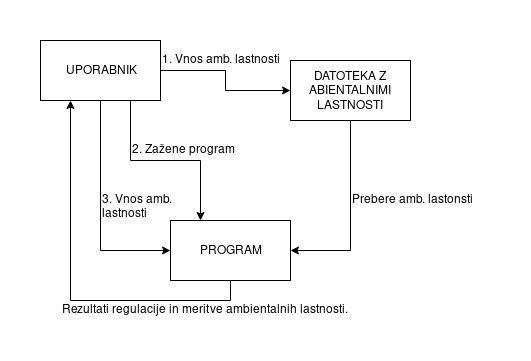
\includegraphics[width=15cm]{diagrami_slike/nivo_sistema.png}
						\end{figure}

					\newpage

					\item Slika 2 Nivo podsistemov - Diagram poteka.	

						\begin{figure}[h]
							\centering
							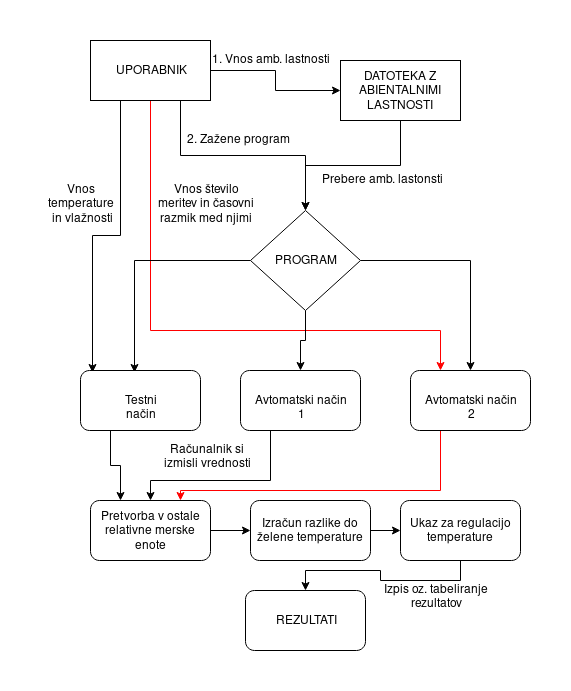
\includegraphics[width=13cm]{diagrami_slike/nivo_podsistemov.png}
						\end{figure}

				\end{itemize}
			
			\subsubsection{Opis procesov}
		
				\begin{itemize}
					\item Program - uporabnik zažene program in mu program omogoči izbiro med dvema načinoma delovanja programa
					\item Testni način - do testnega načina se lahko dostopi samo z argumentom -t ko se program zažene preko cmd.
						Testni način omogoča da uporabnik vnese temperaturo in vlažnost in na to avtmocki program nadaljue z izvajanjem
						ostalih izračunov.
					\item Avtomatski način 1 - izmisli vse potrebne veličine ki jih uporabnik vnaša v Testnem načinu oziroma simulira in
						na koncu prikaže rezultate pretvorb in izračunov.
					\item Avtomatski način 2 - uporabnik vnese število meritev in časovni razmik med njimi, ostale vrednosti program
						izmisli kot v Avtomatske načinu 1 in na koncu prikaže rezultate pretvorb in izračunov.
					\item Pretvorba v ostale relativne merske enote - program samo pretvori vneseno temperaturo v ostale merske enote.
					\item Izračun razlike do želene temperature - program izračuna razliko med vneseno temperaturo v programu 
						(dejanska temp. v prostoru) in želeno temperaturo ki jo prebere iz datoteke. Razlika temperature se izračuna
						v vseh enotah za temperaturo.
					\item Ukaz za regulacijo temperature - regulira temperaturo.
					\item Rezultati - rezultati so podani v obliki tabele.
				\end{itemize}


		\subsection{Opis podatkovnih tokov in terminatorjev}

			\subsubsection{Podatkovni slovar za sliko 2}

			\begin{center}
			\begin{tabular}{|c|c|c|c|c|c|}
					\hline 
					\rowcolor{purple!30!} &Ime podatka&Atribut&Tip&Veljavno območje&Opomba\\
					\hline
					1&Temperatura&&float&10 do 40&oblike: 14.36, 13.00\\
					\hline
					2&Vlažnost&&float&30 do 60&oblike: 42.5, 53.0\\
					\hline
					3&Število meritev&&integer&&\\
					\hline
					4&Časovni razmik&&integer&&\\
					\hline
			\end{tabular}
			\end{center}

			\subsubsection{Opis terminatorjev}
			{%\renewcommand{\arraystretch}{1.5}	
			\begin{center}
			\begin{tabular}{|c|c|}
					\hline
					\rowcolor{purple!30!}Ime terminatorja&Opomba \\
					\hline
					Uporabnik&Oseba ki uporablja program \\
					\hline
					Datoteka z ambientalnimi lastnosti & \thead{Vsaka ambientalna lastnost je napisana v novo vrstico \\ 
															Primer: TEMPERATURA: 25 \\ \hspace{0.7cm} VLAZNOST: 35 ...}  \\
					\hline
			\end{tabular}
			\end{center}
			}

		\subsection{Podroben opis in indeksiranje funkcij in drugih zahtev ki jih je potrebno implementirati}

			\subsubsection{Interaktivni vnos}
				\qquad \qquad Vnos temperature, vlažnosti, število meritev in časovni razmik preko tipkovnice.

			\subsubsection{Branje iz datoteke}
				\qquad \qquad Program mora znati prebrat ambientalne lastnosti iz datoteke.

			\subsubsection{Pretvorba temperature v ostale relativne merske enote}
				\qquad \qquad Program mora pretvoriti vneseno temperaturo v ostale merske enote za temperaturo.

			\subsubsection{Izračun razlike do želene temperature}
				\qquad \qquad Program mora izračunati razliko temperature v vseh mernih enotah.
			
			\subsubsection{Povprečna vrednost meritev in povprečno odstopanje}
				\qquad \qquad Program mora izračunati povprečno vrednost meritev ter povprečno odstopanje od 
				želenih vrednosti za posamezne parametre.

			\subsubsection{Tabeliranje rezultatov}
				\qquad \qquad Program mora tabelirati dobijenih rezultatov odvisnih od našega vnosa vrednosti.

			\subsubsection{Kontrola vhodnih podatkov}
				\qquad \qquad Program mora prepoznati in upozoriti če vnesemo ne veljavni tip podatka preko tipkovnice.

			\subsubsection{Testni način}
				\qquad \qquad Program mora imati vgrajen testni način delovanja ki je dostopen samo preko argumenta
				ki ga dodamo ko zaženemo program. Testni način nam omogoča vpis dodatnih podatkov za natačno testiranje.
		

		\subsection{Zunanji videz}

			\subsubsection{Glavni meni}

				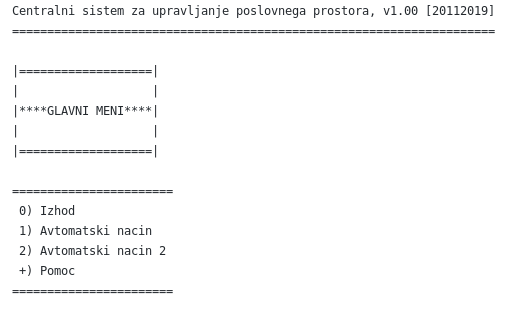
\includegraphics[width=11cm]{diagrami_slike/gl_meni.png}

			\subsubsection{Avtomatski način}

				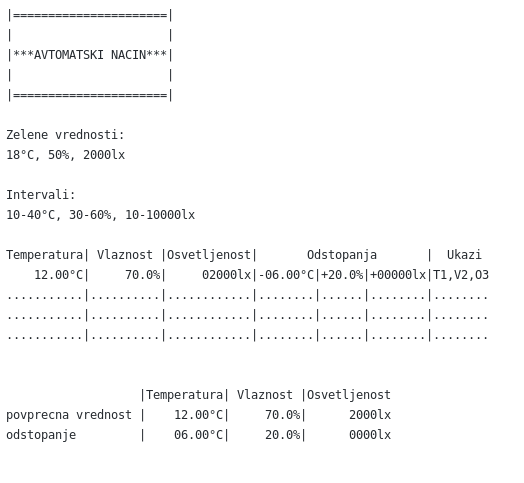
\includegraphics[width=11cm]{diagrami_slike/avt_nac.png}

\newpage

			\subsubsection{Avtomatski način 2}

				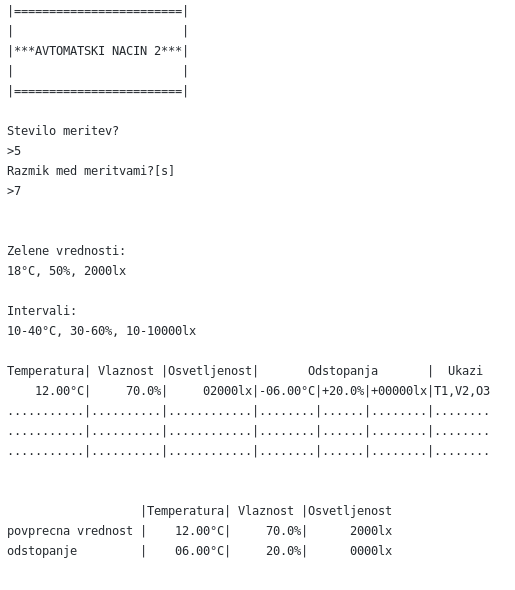
\includegraphics[width=10cm]{diagrami_slike/avt_nac2.png}

			\subsubsection{Pomoč}

				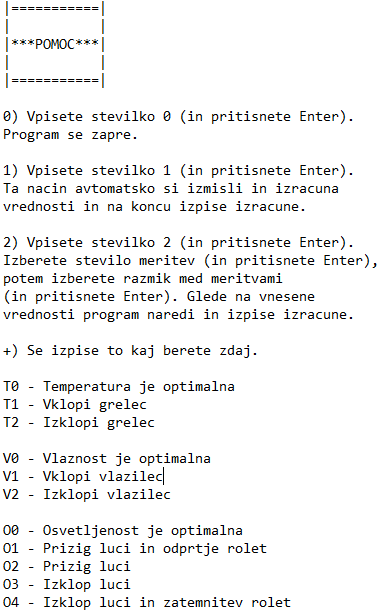
\includegraphics[width=7.3cm]{diagrami_slike/pomoc.png}

			\subsubsection{Testni način}
		
				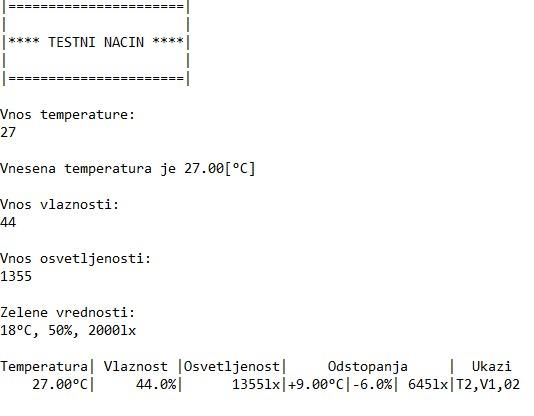
\includegraphics[width=8.2cm]{diagrami_slike/testni_nacin.jpg}

		\subsection{Opis funkcij, ki bodo najprej implementirane}

			\begin{itemize}
				\item Glavni meni
						\begin{itemize}
							\item Prebere vrednosti iz datoteke
							\item Interaktivna izbira načina delovanja
						\end{itemize}
				\item Avtomatski način
						\begin{itemize}
							\item Program si izmisli vrednosti
							\item Izračun odstopanja od želene vrednosti
							\item Ukaz za popravek
							\item Tabeliranje izračunane vrednosti
							\item Izračun povprečno vrednost meritev
							\item Izračun povprečno odstopanje od želenih vrednosti za posamezne parametre
						\end{itemize}
				\item Avtomatski način 2
						\begin{itemize}
							\item Interaktivni vnos za število meritev in časovni razmik med njimi
							\item Način izračuna in izpisa je enaki kot v Avtomatske načinu
						\end{itemize}
				\item Izhod
						\begin{itemize}
							\item Program se zapre
						\end{itemize}
			\end{itemize}

		\subsection{Prevzemni kriterij}

			\begin{itemize}
				\item Program mora biti dokumentiran skladno s standardom CVVS-2/2000
				\item Program mora biti preverjen na najmanj 15 testnih primerih. 
				Naročnik bo pripravil tri svoje testne primere, ki ne smejo pokazati na prisotnost večjih hib.
			\end{itemize}

\newpage

	\section{Testni primeri}

		\subsection{Povzetek}

		\qquad Na podlagi naročnikovih zahtev in Plana projekta, je bil izdelan ta dokument, ki natančno definira 
		postopek testiranja in testne primere. Dokument je  uporaben  za  evalvacijo  prototipa
		in  za  testiranje  kompletnega  programa.  Rezultati  testiranja  so  opisani 
		v Poročilu o preverjanju.

		\subsection{Identifikacija objektov, na katere se testni vzorci nanašajo}

		\qquad Testni primeri se nanašajo na csuppv0\_0\_20112019.exe in csuppv1\_0\_20112019.exe

		\subsection{Opis testnih primerov}

		\qquad Tvoreni so 17 testnih primerov v 3 kategorije, ki bodo za testiranje programa v1.0.

		\subsection{Opis testnega postopka}

		\qquad V okolju MS Windows odpremo datoteko v katro se nahaja program csuppvX\_Y\_DDMMYYYY.exe,
		z dvoklikom na miško zaženemo program in začnemo interaktivno vpisovati testne primere preko 
		tipkovnice. 

		\ V primeru testiranja testnega načina odpremo okno command prompt(cmd.exe) in z
		pomočjo ukaza \textbf{cd ime\_datoteke\textbackslash} se prestavimo v datoteko v katero se 
		nahaja csuppvX\_Y\_DDMMYYYY.exe in zaženemo program na način \textbf{csuppvX\_Y\_DDMMYYYY.exe -t}.

\newpage
	
	\begin{landscape}
		\subsection{Identifikacija funkcij in zahtev ter testna matrika}
			\footnotesize
			\centering
			\begin{tabular}{|c|c|c|c|c||c|c|c|c|c|c|c|c|c|c|c|c|c|c|c|c|c|c|c|c|}
			\hline
					Kratek opis&Kompleksnost&\thead{Stopnja \\  kritičnosti}&\thead{Indikator \\ pomembnosti}&\thead{Število \\ testov}
					&T&T&T&T&T&T&T&T&T&T&T&T&T&T&T&T&T&T&T&T\\
			\hline
				Interaktivni vnos&2&3&6&&&&&&&&&&&&&&&&&&&&&\\
				\hline
				Branje iz datoteke&2&3&6&&&&&&&&&&&&&&&&&&&&&\\
				\hline
				Pretvorba temp.&3&2&6&&&&&&&&&&&&&&&&&&&&&\\
				\hline
				Izračun temp. razl.&1&2&2&&&&&&&&&&&&&&&&&&&&&\\
				\hline
				PVM in PO&1&2&2&&&&&&&&&&&&&&&&&&&&&\\
				\hline
				Tabeliranje rezultov&2&2&4&&&&&&&&&&&&&&&&&&&&&\\
				\hline
				Kontrola vh. podat.&3&3&9&&&&&&&&&&&&&&&&&&&&&\\
				\hline
				Testni način&2&1&2&&&&&&&&&&&&&&&&&&&&&\\
				\hline
					Skupaj&&&37(100\%)&&&&&&&&&&&&&&&&&&&&&\\
			\hline

		\end{tabular}

	\end{landscape}
\newpage
		\subsection{Priloga}

			%\subsubsection{Opis vhodne domene}

			%\subsubsection{Opis izhodne domene}

			\subsubsection{Priloga s konkretnimi testni primeri}

			
			\ Preverjanje prisotnosti zahtev:
				\begin{itemize}

					\item TP1-1 Ali je prisotna najbolj kritična funkconalnost?
							Ali je implementiran testni režim?

					\item TP1-2 Ali je vedno prisotna vgrajena pomoč?

					%\item TP1-3 Ali sta zahtevana natančnost in hitrost prisotna?

				\end{itemize}
			\ Preverjanje natančnost in pravilnost izračunov:
				\begin{itemize}
					\item TP2-1 Ali program generira vse pravilne vrednosti za pravilno delovanje Avtomatskega načina?
					\item TP2-2 Ali program izvede zahtevano število meritev za zahtevanega časovnega rezmika ?
					\item TP2-3 Ali program izračuna povprečno vrednost meritev ter povprečno odstopanje od želenih vrednosti za posamezne parametre ?
					\item TP2-4 Ali program pretvori vneseno temperaturo v ostale merske enote ?
					\item TP2-5 Ali program izračuna razliko do želene temperature (v vseh merskih enotah) ?
					\item TP2-6 Ali program pravilno izvede ukaz za regulacijo temperature ?
					\item TP2-7 Ali program pravilno izračuna in izvede ukaze za vlažnost in osvetljenost ? 
					\item TP2-8 Ali program prekine svoje izvajanje na zahtevo uporabnika v Testnem načinu ?
				\end{itemize}
			\ Preverjanje robustnosti vhodnih podatkov:
				\begin{itemize}

					\item TP3-1 Ali program pravilno procesira neveljavne vhodne podatke?
					\item TP3-2 Ali program opozori za vnost temperature izven intervala $(10\ \degree C,40\ \degree C)$
					\item TP3-3 Ali program opozori za vnos vlažnosti izven intervala $(30\%,60\%)$
					\item TP3-4 Ali program opozori za vnos osvetljenosti izven intervala $(10\ lx,10000\ lx)$
					\item TP3-5 Ali program opozori za maksimalno možno število meritev?
					\item TP3-6 Ali program opozori za minimalni ali maksimalni časovni razmik med število meritev?
					\item TP3-7 Ali je program odporen na nepravilni vnos ambientalnih lastnosti v tekstovno datoteko?

				\end{itemize}
			
\newpage

	\begin{landscape}

			\paragraph{Ali je prisotna najbolj kritična funkcionalnost in Testni način ?}
			
			\centering
			
		
			\rowcolors{1}{purple!30!}{}
			\begin{tabular}{|c|c|c|c|}
			
					\hline
					Testni primer&Avtor&Verzija&Projekt \\
					\hline \hline
					TP1-1& Anton Zhezhov&V1.0&CSUPP \\
					\hline

			\end{tabular}
			
			\vspace{0.3cm}
			
			\rowcolors{1}{purple!30!}{}
			
			\begin{tabular}{|c|c|c|c|c|c|}
				\hline
				Začetno stanje&Namen&Konf. sistema&Strategija&Opomba&Odvisnost od drugih testov \\
				\hline \hline
				\thead{Okno Command Prompt \\ 
						(odprto na lokaciji \\
						mapao programa).}&\thead{Ali je prisotna najbolj \\ 
											kritična funkcionalnost \\ 
											in Testni način ?}& Windows 10 Pro&\thead{Preverjanje \\ 
																						prisotnosti zahtev.}&\thead{Testni način \\ 
																											je za demonstracijo
																											\\delovanje programa.}&Ni nobene odvisnosti. \\
				\hline
			\end{tabular}

			\vspace{0.3cm}

			\rowcolors{1}{purple!30!}{}
			
			\begin{tabular}{|c|c|c|C{5.5cm}|c|c|}
					\hline
					Korak&Akcija/Ime vhodne spremenjljivke&Vrednost&Pričekovana reakcija/vrednost&Opomba&Opomba za testno poročilo \\
					\hline \hline
					1&csuppvX\_Y\_DDMMYYYY.exe -t&&\small{Izpis da smo v Testnem  
														načinu, pod izpisa, interaktivni 
														vnos za temeraturo.}&&\\
					\hline
					2&Vpišemo temperaturo&37&\small{Izpis vnesene temperature   
													z enoto in pretvorba v ostale merske 
													enote, pod izpisa, 
													interaktivni vnost za vlažnost.}&&\\
					3&Vpišemo vlažnost&48&\small{Pod vpisano vrednost,
												interaktivni vnost za osvetljenost.}&&\\
					\hline
					4&Vpišemo osvetljenost&5243&\small{Pod vpisano vrednost se izpišejo
													želene vrednosti se izvedejo 
													potrebni izračuni in tabeliranje.}&&\\
					\hline
					5&Zahtevamo prekinitev izračunov&p&Izračuni in tabeliranje se prekineta.&&\\

					\hline
					6&Izberemo ponovni vnos vrednosti&*&\small{Izpis da smo v Testnem 
														načinu, pod izpisa, interaktivni 
														vnos za temeraturo.}&&\\
					\hline
					7&Korake od 2 do 5&&\small{Pričekujemo enaki 
										način delovanje
										kot v korake od 2 do 5.}&&\\ 
					\hline
					8&Želimo izhod&0&\small{Okno Command Prompt
											(odprto na lokaciji
											mapao programa).}&&\\
					\hline
			\end{tabular}


			
	\end{landscape}

\newpage

	\begin{landscape}
	
		\paragraph{Ali je vedno prisotna vgrajena pomoč ?}
			
			\centering
			
		
			\rowcolors{1}{purple!30!}{}
			\begin{tabular}{|c|c|c|c|}
			
					\hline
					Testni primer&Avtor&Verzija&Projekt \\
					\hline \hline
					TP1-2& Anton Zhezhov&V1.0&CSUPP \\
					\hline

			\end{tabular}
			
			\vspace{0.3cm}
			
			\rowcolors{1}{purple!30!}{}
			
			\begin{tabular}{|c|c|c|c|c|c|}
				\hline
				Začetno stanje&Namen&Konf. sistema&Strategija&Opomba&Odvisnost od drugih testov \\
				\hline \hline
				\thead{Okno Command Prompt \\ 
						(odprto na lokaciji \\
						mapao programa).}&\thead{Ali je vedno prisotna \\ 
											vgrajena pomoč ? \\}& Windows 10 Pro&\thead{Preverjanje \\ 
																						prisotnosti zahtev.}&\thead{Testni način \\ 
																											je za demonstracijo
																											\\delovanje programa.}&Ni nobene odvisnosti. \\
				\hline
			\end{tabular}

			\vspace{0.3cm}

			\rowcolors{1}{purple!30!}{}

			\begin{tabular}{|c|c|c|C{5.5cm}|c|c|}
					\hline
					Korak&Akcija/Ime vhodne spremenjljivke&Vrednost&Pričekovana reakcija/vrednost&Opomba&Opomba za testno poročilo \\
					\hline \hline
					1&csuppvX\_Y\_DDMMYYYY.exe -t&&\small{Izpis da smo v Testnem  
														načinu, pod izpisa, interaktivni 
														vnos za temeraturo.}&&\\
					\hline
					2&Zahtevamo pomoč&+&Izpis pomoči za to polje&&\\
					\hline
					3&Vpišemo temperaturo&37&\small{Izpis vnesene temperature   
													z enoto in pretvorba v ostale merske enote, 
													pod izpisa, 
													interaktivni vnost za vlažnost.}&&\\
					\hline
					4&Zahtevamo pomoč&+&Izpis pomoči za to polje&&\\
					\hline
					5&Vpišemo vlažnost&48&\small{Pod vpisano vrednost,
												interaktivni vnost za osvetljenost.}&&\\
					\hline
					6&Zahtevamo pomoč&+&Izpis pomoči za to polje&&\\
					\hline
					7&Vpišemo osvetljenost&5243&\small{Pod vpisano vrednost se izpišejo
													želene vrednosti se izvedejo 
													potrebni izračuni in tabeliranje.}&&\\
					\hline
					8&Zahtevamo pomoč&+&Izpis pomoči za to polje&&\\
					\hline
					9&Izberemo ponovni vnos vrednosti&*&\small{Izpis da smo v Testnem 
														načinu, pod izpisa, interaktivni 
														vnos za temeraturo.}&&\\
					\hline
					10&Korake od 2 do 9&&\small{Pričekujemo enaki 
										način delovanje
										kot v korake od 2 do 9.}&&\\ 
					\hline
					11&Želimo izhod&0&\small{Okno Command Prompt
											(odprto na lokaciji
											mapao programa).}&&\\
					\hline
			\end{tabular}

	\end{landscape}

\newpage

	\begin{landscape}
	
		\paragraph{Ali program generira vse pravilne vrednosti za pravilno delovanje Avtomatskega načina ?}
			
			\centering
			
		
			\rowcolors{1}{purple!30!}{}
			\begin{tabular}{|c|c|c|c|}
			
					\hline
					Testni primer&Avtor&Verzija&Projekt \\
					\hline \hline
					TP2-1& Anton Zhezhov&V1.0&CSUPP \\
					\hline

			\end{tabular}
			
			\vspace{0.3cm}
			
			\rowcolors{1}{purple!30!}{}
			
			\begin{tabular}{|c|c|c|c|c|c|}
				\hline
				Začetno stanje&Namen&Konf. sistema&Strategija&Opomba&Odvisnost od drugih testov \\
				\hline \hline
				\thead{Okno Command Prompt \\ 
						(odprto na lokaciji \\
						mapao programa).}&\thead{Generiranje \\  
												pravilne vrednosti.}& Windows 10 Pro&\thead{Preverjanje natančnost \\  
																						 in pravilnost.}&Ni opomb.&Ni nobene odvisnosti. \\
				\hline
			\end{tabular}

			\vspace{0.3cm}

			\rowcolors{1}{purple!30!}{}

			\begin{tabular}{|c|c|c|C{5.5cm}|c|c|}
					\hline
					Korak&Akcija/Ime vhodne spremenjljivke&Vrednost&Pričekovana reakcija/vrednost&Opomba&Opomba za testno poročilo \\
					\hline \hline
					1&csuppvX\_Y\_DDMMYYYY.exe&&\small{Izpis da smo v Glavni meni,  
														pod izpisom, interaktivni
														vnos za izbiro načina delovanja.}&&\\
					\hline
					2&Izberemo Avtomatski način&1&\small{Izpis da smo v Avtomatskem
													načinu, izpis želenih vrednost, 
													izpis intervalov, tabeliranje, 
													izpis povprečne vrednosti in odstopanje.}&&\\
					\hline
					3&Izberemo Avtomatski način &1&\small{Pričekujemo enaki izpis kot prej.}&&\\
					
					\hline
					4&Zahtevamo izhod&0&Okno Command Prompt
										(odprto na lokaciji 
										mapao programa).&&\\
					\hline
			\end{tabular}

	\end{landscape}

\newpage

	\begin{landscape}
	
		\paragraph{Ali program izvede zahtevano število meritev za zahtevanega časovnega razmika ?}
			
			\centering
			
		
			\rowcolors{1}{purple!30!}{}
			\begin{tabular}{|c|c|c|c|}
			
					\hline
					Testni primer&Avtor&Verzija&Projekt \\
					\hline \hline
					TP2-2& Anton Zhezhov&V1.0&CSUPP \\
					\hline

			\end{tabular}
			
			\vspace{0.3cm}
			
			\rowcolors{1}{purple!30!}{}
			
			\begin{tabular}{|c|c|c|c|c|c|}
				\hline
				Začetno stanje&Namen&Konf. sistema&Strategija&Opomba&Odvisnost od drugih testov \\
				\hline \hline
				\thead{Okno Command Prompt \\ 
						(odprto na lokaciji \\
						mapao programa).}&\thead{Število meritev in\\  
												časovni razmik.}& Windows 10 Pro&\thead{Preverjanje natančnost \\  
																						 in pravilnost.}&Ni opomb.&Ni nobene odvisnosti. \\
				\hline
			\end{tabular}

			\vspace{0.3cm}

			\rowcolors{1}{purple!30!}{}

			\begin{tabular}{|c|c|c|C{5.5cm}|c|c|}
					\hline
					Korak&Akcija/Ime vhodne spremenjljivke&Vrednost&Pričekovana reakcija/vrednost&Opomba&Opomba za testno poročilo \\
					\hline \hline
					1&csuppvX\_Y\_DDMMYYYY.exe&&\small{Izpis da smo v Glavni meni,  
														pod izpisom, interaktivni
														vnos za izbiro načina delovanja.}&&\\
					\hline
					2&Izberemo Avtomatski način&1&\small{Izpis da smo v Avtomatskem
													načinu, izpis želenih vrednost, 
													izpis intervalov, tabeliranje, 
													izpis povprečne vrednosti in odstopanje.}&&\\
					\hline
					3&Izberemo Avtomatski način &1&\small{Pričekujemo enaki izpis kot prej
															in 100 meritve na vsake 3 sekunde v tabelo.}&&\\
					
					\hline
					4&Zahtevamo izhod&0&Okno Command Prompt
										(odprto na lokaciji 
										mapao programa).&&\\
					\hline
			\end{tabular}

	\end{landscape}

\newpage

	\begin{landscape}
	
		\paragraph{Ali program izračuna povprečno vrednost meritev ter povprečno odstopanje od želenih vrednosti za posamezne parametre ?}
			
			\centering
			
		
			\rowcolors{1}{purple!30!}{}
			\begin{tabular}{|c|c|c|c|}
			
					\hline
					Testni primer&Avtor&Verzija&Projekt \\
					\hline \hline
					TP2-3& Anton Zhezhov&V1.0&CSUPP \\
					\hline

			\end{tabular}
			
			\vspace{0.3cm}
			
			\rowcolors{1}{purple!30!}{}
			
			\begin{tabular}{|c|c|c|c|c|c|}
				\hline
				Začetno stanje&Namen&Konf. sistema&Strategija&Opomba&Odvisnost od drugih testov \\
				\hline \hline
				\thead{Okno Command Prompt \\ 
						(odprto na lokaciji \\
						mapao programa).}&\thead{Povprečna vrednost meritev \\  
												in povprečno odstopanje.}& Windows 10 Pro&\thead{Preverjanje natančnost \\  
																						 in pravilnost.}&Ni opomb.&Ni nobene odvisnosti. \\
				\hline
			\end{tabular}

			\vspace{0.3cm}

			\rowcolors{1}{purple!30!}{}

			\begin{tabular}{|c|c|c|C{5.5cm}|c|c|}
					\hline
					Korak&Akcija/Ime vhodne spremenjljivke&Vrednost&Pričekovana reakcija/vrednost&Opomba&Opomba za testno poročilo \\
					\hline \hline
					1&csuppvX\_Y\_DDMMYYYY.exe&&\small{Izpis da smo v Glavni meni,  
														pod izpisom, interaktivni
														vnos za izbiro načina delovanja.}&&\\
					\hline
					2&Izberemo Avtomatski način&1&\small{Izpis da smo v Avtomatskem
													načinu, izpis želenih vrednost, 
													izpis intervalov, tabeliranje, 
													izpis povprečne vrednosti in odstopanje.}&&\\
					\hline
					3&Izberemo Avtomatski način &1&\small{Pričekujemo enaki izpis kot prej
															in po tabeli izpis povprečne 
															vrednosti in odstopanje za
															Temp., Vlaž. in Osvetljenost.}&&\\
					
					\hline
					4&Zahtevamo izhod&0&Okno Command Prompt
										(odprto na lokaciji 
										mapao programa).&&\\
					\hline
			\end{tabular}
	\end{landscape}

\newpage

	\begin{landscape}
	
		\paragraph{Ali program pretvori vneseno temperaturo v ostale merske enote ?}
			
			\centering
			
		
			\rowcolors{1}{purple!30!}{}
			\begin{tabular}{|c|c|c|c|}
			
					\hline
					Testni primer&Avtor&Verzija&Projekt \\
					\hline \hline
					TP2-4& Anton Zhezhov&V1.0&CSUPP \\
					\hline

			\end{tabular}
			
			\vspace{0.3cm}
			
			\rowcolors{1}{purple!30!}{}
			
			\begin{tabular}{|c|c|c|c|c|c|}
				\hline
				Začetno stanje&Namen&Konf. sistema&Strategija&Opomba&Odvisnost od drugih testov \\
				\hline \hline
				\thead{Okno Command Prompt \\ 
						(odprto na lokaciji \\
						mapao programa).}&\thead{Pretvorba temperature \\  
												v ostale merske enote.}& Windows 10 Pro&\thead{Preverjanje natančnost \\  
																						 in pravilnost.}&Ni opomb.&Ni nobene odvisnosti. \\
				\hline
			\end{tabular}

			\vspace{0.3cm}

			\rowcolors{1}{purple!30!}{}

			\begin{tabular}{|c|c|c|C{5.9cm}|c|c|}
					\hline
					Korak&Akcija/Ime vhodne spremenjljivke&Vrednost&Pričekovana reakcija/vrednost&Opomba&Opomba za testno poročilo \\
					\hline \hline
					1&csuppvX\_Y\_DDMMYYYY.exe -t&&\small{Izpis da smo v Testni način,  
														pod izpisom, interaktivni
														vnos za temperaturo.}&&\\
					\hline
					2&Vpišemo temperaturo&300.15&\small{Izpis da je vnesena 
														temperatura 300.15[K] in izpis
														pretvorbe v ostale merske enote, potem
														vnos nadaljuje kot v TP1-1 od koraka 3.}&&\\
					\hline
					3&Vpišemo temperaturo&308.15&\small{Izpis da je vnesena 
														temperatura 308.15[K] in izpis
														pretvorbe v ostale merske enote, potem
														vnos nadaljuje kot v TP1-1 od koraka 3.}&&\\

					\hline
					4&Zahtevamo izhod&0&Okno Command Prompt
										(odprto na lokaciji 
										mapao programa).&&\\
					\hline
			\end{tabular}
	\end{landscape}

\newpage

	\begin{landscape}
	
		\paragraph{Ali program izračuna razliko do želene temperature ?}
			
			\centering
			
		
			\rowcolors{1}{purple!30!}{}
			\begin{tabular}{|c|c|c|c|}
			
					\hline
					Testni primer&Avtor&Verzija&Projekt \\
					\hline \hline
					TP2-5& Anton Zhezhov&V1.0&CSUPP \\
					\hline

			\end{tabular}
			
			\vspace{0.3cm}
			
			\rowcolors{1}{purple!30!}{}
			
			\begin{tabular}{|c|c|c|c|c|c|}
				\hline
				Začetno stanje&Namen&Konf. sistema&Strategija&Opomba&Odvisnost od drugih testov \\
				\hline \hline
				\thead{Okno Command Prompt \\ 
						(odprto na lokaciji \\
						mapao programa).}&\thead{Izračun razlike do\\  
											želene temperature.}& Windows 10 Pro&\thead{Preverjanje natančnost \\  
																						 in pravilnost.}&Ni opomb.&Ni nobene odvisnosti. \\
				\hline
			\end{tabular}

			\vspace{0.3cm}

			\rowcolors{1}{purple!30!}{}

			\begin{tabular}{|c|c|c|C{5.9cm}|c|c|}
					\hline
					Korak&Akcija/Ime vhodne spremenjljivke&Vrednost&Pričekovana reakcija/vrednost&Opomba&Opomba za testno poročilo \\
					\hline \hline
					1&csuppvX\_Y\_DDMMYYYY.exe -t&&\small{Izpis da smo v Testni način,  
														pod izpisom, interaktivni
														vnos za temperaturo.}&&\\
					\hline
					2&Vpišemo temperaturo&300.15&\small{Izpis da je vnesena 
														temperatura 300.15[K] in izpis
														pretvorbe v ostale merske enote, potem
														vnos nadaljuje kot v TP1-1 koraka 3 in 4 in 
														se izpiše tabela z izračunane razlike .}&&\\
					\hline
					3&Vpišemo temperaturo&308.15&\small{Izpis da je vnesena 
														temperatura 308.15[K] in izpis
														pretvorbe v ostale merske enote, potem
														vnos nadaljuje kot v TP1-1 koraka 3 in 4 in 
														se izpiše tabela z izračunane razlike.}&&\\

					\hline
					4&Zahtevamo izhod&0&Okno Command Prompt
										(odprto na lokaciji 
										mapao programa).&&\\
					\hline
			\end{tabular}
	\end{landscape}

\newpage

	\begin{landscape}
	
		\paragraph{Ali program pravilno izvede ukaze za regulacijo ?}
			
			\centering
			
		
			\rowcolors{1}{purple!30!}{}
			\begin{tabular}{|c|c|c|c|}
			
					\hline
					Testni primer&Avtor&Verzija&Projekt \\
					\hline \hline
					TP2-6& Anton Zhezhov&V1.0&CSUPP \\
					\hline

			\end{tabular}
			
			\vspace{0.3cm}
			
			\rowcolors{1}{purple!30!}{}
			
			\begin{tabular}{|c|c|c|c|c|c|}
				\hline
				Začetno stanje&Namen&Konf. sistema&Strategija&Opomba&Odvisnost od drugih testov \\
				\hline \hline
				\thead{Okno Command Prompt \\ 
						(odprto na lokaciji \\
						mapao programa).}&\thead{Ukazi za \\  
											regulacijo temperature.}& Windows 10 Pro&\thead{Preverjanje natančnost \\  
																						 in pravilnost.}&Ni opomb.&Ni nobene odvisnosti. \\
				\hline
			\end{tabular}

			\vspace{0.3cm}

			\rowcolors{1}{purple!30!}{}

			\begin{tabular}{|c|c|c|C{5.9cm}|c|c|}
					\hline
					Korak&Akcija/Ime vhodne spremenjljivke&Vrednost&Pričekovana reakcija/vrednost&Opomba&Opomba za testno poročilo \\
					\hline \hline
					1&csuppvX\_Y\_DDMMYYYY.exe &&\small{Izpis da smo v Glavni meni,  
														pod izpisom, interaktivni
														vnos za izbiro načina delovanja.}&&\\
					\hline
					2&Izberemo Avtomatski način&1&\small{Enako delovanje kot v primer 
														TP2-1 korak 2 in pričekujemo 
														ukaze za regulacijo v najbolj desnem stolpcu tabele.}&&\\
					\hline
					3&Zahtevamo izhod&0&Okno Command Prompt
										(odprto na lokaciji 
										mapao programa).&&\\
					\hline
			\end{tabular}
	\end{landscape}

\newpage

	\begin{landscape}
	
		\paragraph{Ali program pravilno izvede ukaze za vlažnost in osvetljenost ?}
			
			\centering
			
		
			\rowcolors{1}{purple!30!}{}
			\begin{tabular}{|c|c|c|c|}
			
					\hline
					Testni primer&Avtor&Verzija&Projekt \\
					\hline \hline
					TP2-7& Anton Zhezhov&V1.0&CSUPP \\
					\hline

			\end{tabular}
			
			\vspace{0.3cm}
			
			\rowcolors{1}{purple!30!}{}
			
			\begin{tabular}{|c|c|c|c|c|c|}
				\hline
				Začetno stanje&Namen&Konf. sistema&Strategija&Opomba&Odvisnost od drugih testov \\
				\hline \hline
				\thead{Okno Command Prompt \\ 
						(odprto na lokaciji \\
						mapao programa).}&\thead{Ukazi za regulacijo\\  
											valžnosti in osvetljenosti.}& Windows 10 Pro&\thead{Preverjanje natančnost \\  
																						 in pravilnost.}&Ni opomb.&Ni nobene odvisnosti. \\
				\hline
			\end{tabular}

			\vspace{0.3cm}

			\rowcolors{1}{purple!30!}{}

			\begin{tabular}{|c|c|c|C{5.9cm}|c|c|}
					\hline
					Korak&Akcija/Ime vhodne spremenjljivke&Vrednost&Pričekovana reakcija/vrednost&Opomba&Opomba za testno poročilo \\
					\hline \hline
					1&csuppvX\_Y\_DDMMYYYY.exe &&\small{Izpis da smo v Glavni meni,  
														pod izpisom, interaktivni
														vnos za izbiro načina delovanja.}&&\\
					\hline
					2&Izberemo Avtomatski način&1&\small{Enako delovanje kot v primer 
														TP2-1 korak 2 in pričekujemo 
														ukaze za regulacijo v najbolj desnem stolpcu tabele.}&&\\
					\hline
					3&Zahtevamo izhod&0&Okno Command Prompt
										(odprto na lokaciji 
										mapao programa).&&\\
					\hline
			\end{tabular}
	\end{landscape}

\newpage

	\begin{landscape}
	
		\paragraph{Ali program prekine svoje izvajanje na zahtevo uporabnika v Testnem načinu ?}
			
			\centering
			
			\rowcolors{1}{purple!30!}{}
			\begin{tabular}{|c|c|c|c|}
			
					\hline
					Testni primer&Avtor&Verzija&Projekt \\
					\hline \hline
					TP2-8& Anton Zhezhov&V1.0&CSUPP \\
					\hline

			\end{tabular}
			
			\vspace{0.3cm}
			
			\rowcolors{1}{purple!30!}{}
			
			\begin{tabular}{|c|c|c|c|c|c|}
				\hline
				Začetno stanje&Namen&Konf. sistema&Strategija&Opomba&Odvisnost od drugih testov \\
				\hline \hline
				\thead{Okno Command Prompt \\ 
						(odprto na lokaciji \\
						mapao programa).}&\thead{Prekinitev \\  
											izvajanja.}& Windows 10 Pro&\thead{Preverjanje natančnost \\  
																						 in pravilnost.}&Ni opomb.&Ni nobene odvisnosti. \\
				\hline
			\end{tabular}

			\vspace{0.3cm}

			\rowcolors{1}{purple!30!}{}

			\begin{tabular}{|c|c|c|C{5.9cm}|c|c|}
					\hline
					Korak&Akcija/Ime vhodne spremenjljivke&Vrednost&Pričekovana reakcija/vrednost&Opomba&Opomba za testno poročilo \\
					\hline \hline
					1&csuppvX\_Y\_DDMMYYYY.exe -t &&\small{Izpis da smo v Testni način,  
														pod izpisom, interaktivni
														vnos za temperaturo.}&&\\
					\hline
					2&Vnesemo temperaturo&30&\small{Enako delovanje kot v primer 
														TP1-1 od koraka 2 do koraka 4.}&&\\
					\hline
					3&Zahtevamo prekinitev izračunov&p&Izračuni in tabeliranje se prekineta.&&\\
					\hline
					4&Zahtevamo izhod&0&Okno Command Prompt
										(odprto na lokaciji 
										mapao programa).&&\\
					\hline
			\end{tabular}
	\end{landscape}

\newpage

	\begin{landscape}
	
			\paragraph{Procesiranje neveljavnih vhodnih podatkov (od TP3-1 do TP3-6).}
			
			\centering
			
			\rowcolors{1}{purple!30!}{}
			\begin{tabular}{|c|c|c|c|}
			
					\hline
					Testni primeri&Avtor&Verzija&Projekt \\
					\hline \hline
					TP3-1 do TP3-6& Anton Zhezhov&V1.0&CSUPP \\
					\hline

			\end{tabular}
			
			\vspace{0.3cm}
			
			\rowcolors{1}{purple!30!}{}
			
			\begin{tabular}{|c|c|c|c|c|c|}
				\hline
				Začetno stanje&Namen&Konf. sistema&Strategija&Opomba&Odvisnost od drugih testov \\
				\hline \hline
				\thead{Okno Command Prompt \\ 
						(odprto na lokaciji \\
						mapao programa).}&\thead{Procesiranje \\  
											neveljavnih podatkov.}& Windows 10 Pro&\thead{Preverjanje robustnosti \\  
																						 vhodnih podatkov.}&Ni opomb.&Ni nobene odvisnosti. \\
				\hline
			\end{tabular}

			\vspace{0.3cm}

			\rowcolors{1}{purple!30!}{}

			\begin{tabular}{|c|c|c|C{10cm}|c|c|}
					\hline
					Korak&Akcija/Ime vhodne spremenjljivke&Vrednost&Pričekovana reakcija/vrednost&Opomba&OTP \\
					\hline \hline
					1&csuppvX\_Y\_DDMMYYYY.exe -t &&\small{Izpis da smo v Testni način,  
														pod izpisom, interaktivni
														vnos za temperaturo.}&&\\
					\hline
					2&Vnesemo temperaturo&-120000.12&\small{Opozotilo za neveljavno vrednost 
														temperature, potem se pojavi ponovni 
														interaktivni vnos za temperaturo.}&&\\
					\hline
					3&Vnesemo vlažnost &172.8&\small{Opozotilo za neveljavno vrednost 
														vlažnsti, potem se pojavi ponovni 
														interaktivni vnos za vlažnost.}&&\\
					\hline
					4&Vnesemo osvetljenost &-127a&\small{Opozotilo za neveljavno vrednost 
														osvetljenosti, potem se pojavi ponovni 
														interaktivni vnos za osvetljenost.}&&\\
					\hline
					5&Zahtevamo prekinitev izračunov&p&Izračuni in tabeliranje se prekineta.&&\\
					\hline
					6&Zahtevamo izhod&0&Okno Command Prompt
										(odprto na lokaciji 
										mapao programa).&&\\
					\hline
					7&csuppvX\_Y\_DDMMYYYY.exe&&\small{Izpis da smo v Glavni meni,  
														pod izpisom, interaktivni
														vnos za izbiro načina delovanja.}&&\\
					\hline
					8&Izberemo Avtomatski način 2&2&\small{Izpis za interaktivni vnost število
															meritev.}&&\\
					\hline
					9&Vpišemo število meritev&10.23e-18&\small{Opozorilo za neveljavno vrednost
																meritve, potem se pojavi ponovni 
																interaktivni vnos za številio meritve.}&&\\
					\hline
					10&Vpišemo časovni razmik&65*87&\small{Opozorilo za neveljavno vrednost
															razmika, potem se pojavi ponovni 
															interaktivni vnos za časovni razmik in tabeliranje.}&&\\
					\hline
					11&Zahtevamo ponovno izbiro načina delovanja&¸&\small{Opozorilo za neveljavno vrednost za izbor načina 
																		delovanja, potem se pojavi ponovni 
																		interaktivni vnos za izbiro.}&&\\
					\hline
					12&Zahtevamo izhod&ž&\small{Opozorilo za neveljavno komando za izhod, potem se 
												program vrne v prejšno stanje v kero je bil.} &&\\
					\hline
					13&Zahtevamo izhod&0&Okno Command Prompt
										(odprto na lokaciji 
										mapao programa).&&\\
					\hline
			\end{tabular}
	\end{landscape}

\newpage

	\begin{landscape}
	
			\paragraph{Ali je program odporen na nepravilni vnos ambientalnih lastnosti v datoteki ?}
			
			\centering
			
			\rowcolors{1}{purple!30!}{}
			\begin{tabular}{|c|c|c|c|}
			
					\hline
					Testni primer&Avtor&Verzija&Projekt \\
					\hline \hline
					TP3-7& Anton Zhezhov&V1.0&CSUPP \\
					\hline

			\end{tabular}
			
			\vspace{0.3cm}
			
			\rowcolors{1}{purple!30!}{}
			
			\begin{tabular}{|c|c|c|c|c|c|}
				\hline
				Začetno stanje&Namen&Konf. sistema&Strategija&Opomba&Odvisnost od drugih testov \\
				\hline \hline
				\thead{Okno Command Prompt \\ 
						(odprto na lokaciji \\
						mapao programa).}&\thead{Procesiranje \\  
											neveljavnih podatkov.}& Windows 10 Pro&\thead{Preverjanje robustnosti \\  
																						 vhodnih podatkov.}&Ni opomb.&Ni nobene odvisnosti. \\
				\hline
			\end{tabular}

			\vspace{0.3cm}

			\rowcolors{1}{purple!30!}{}

			\begin{tabular}{|c|c|c|C{10cm}|c|c|}
					\hline
					Korak&Akcija/Ime vhodne spremenjljivke&Vrednost&Pričekovana reakcija/vrednost&Opomba&OTP \\
					\hline \hline
					1&csuppvX\_Y\_DDMMYYYY.exe -t &&\small{Izpis da smo v Testni način,  
														pod izpisom opozorilo da 
														tekstovna datoteka vsebuje neveljavni tip  podatkov.}&&\\
					\hline
					2&csuppvX\_Y\_DDMMYYYY.exe&&\small{Izpis da smo v Glavni meni,  
														pod izpisom, opozorilo da tekstovna datoteka vsebuje
														neveljavni tip podatkov.}&&\\
					\hline
			\end{tabular}
	\end{landscape}

\end{document}
